\documentclass{article}

\usepackage[T1]{fontenc}
\usepackage{mathptmx}
\usepackage{fancyhdr} 
\usepackage{url}
\usepackage{graphicx}
\usepackage{tikz}
\usepackage{listings}
\usepackage{color}
\usepackage{tikzpagenodes}
\usepackage{lipsum}
\usepackage{capt-of}
\usepackage{floatrow}
\usepackage{subfig}
\usepackage[latin1]{inputenc}


\floatsetup[figure]{style=plain,subcapbesideposition=center}

\definecolor{dkgreen}{rgb}{0,0.6,0}
\definecolor{gray}{rgb}{0.5,0.5,0.5}
\definecolor{mauve}{rgb}{0.58,0,0.82}

\lstset{frame=tb,
  language=Java,
  aboveskip=3mm,
  belowskip=3mm,
  showstringspaces=false,
  columns=flexible,
  basicstyle={\small\ttfamily},
  numbers=none,
  numberstyle=\tiny\color{gray},
  keywordstyle=\color{blue},
  commentstyle=\color{dkgreen},
  stringstyle=\color{mauve},
  breaklines=true,
  breakatwhitespace=true,
  tabsize=3
}

\usepackage{setspace}
\usetikzlibrary{calc,trees,positioning,arrows,chains,shapes.geometric,%
    decorations.pathreplacing,decorations.pathmorphing,shapes,%
    matrix,shapes.symbols,fit}
    
\tikzstyle{decision} = [diamond, draw, fill=blue!20, 
    text width=4.5em, text badly centered, node distance=3cm, inner sep=0pt]
\tikzstyle{block} = [rectangle, draw, fill=blue!20, 
    text width=5em, text centered, rounded corners, minimum height=4em]
\tikzstyle{line} = [draw, -latex']
\tikzstyle{cloud} = [draw, ellipse,fill=red!20, node distance=3cm,
    minimum height=2em]

\tikzset{
%>=stealth',
  punktchain/.style={
    rectangle, 
    rounded corners, 
    % fill=black!10,
    draw=orange, very thick,
    text width=10em, 
    minimum height=1em, 
    text centered, 
    on chain},
  line/.style={draw, thick, <-},
  element/.style={
    tape,
    top color=white,
    bottom color=blue!50!black!60!,
   minimum width=8em,
    draw=blue!40!black!90, very thick,
    text width=10em, 
    minimum height=1em, 
    text centered, 
    on chain},
  every join/.style={->, thick,shorten >=1pt},
  decoration={brace},
  tuborg/.style={decorate},
  tubnode/.style={midway, right=2pt},
}
\begin{document}

\begin{figure}%[htbp]
\sidesubfloat[]{
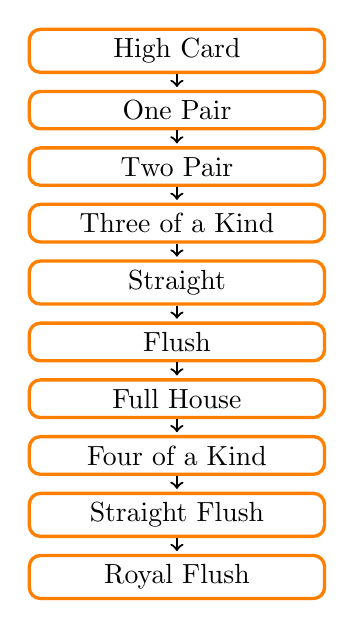
\begin{tikzpicture}
  [node distance=.2cm,
  start chain=going below,]
     \node[punktchain, join](HighCard){High Card};
     \node[punktchain, join](OnePair){One Pair};
     \node[punktchain, join](TwoPair){Two Pair};
     \node[punktchain, join](ThreeofaKind){Three of a Kind};
     \node[punktchain, join](Straight){Straight};
     \node[punktchain, join](Flush){Flush};
     \node[punktchain, join] (FullHouse){Full House};
     \node[punktchain, join] (FourofaKind){Four of a Kind};
     \node[punktchain, join] (StraightFlush){Straight Flush};
     \node[punktchain, join] (RoyalFlush) {Royal Flush}; 

   \end{tikzpicture}
	
}\qquad
\sidesubfloat[]{
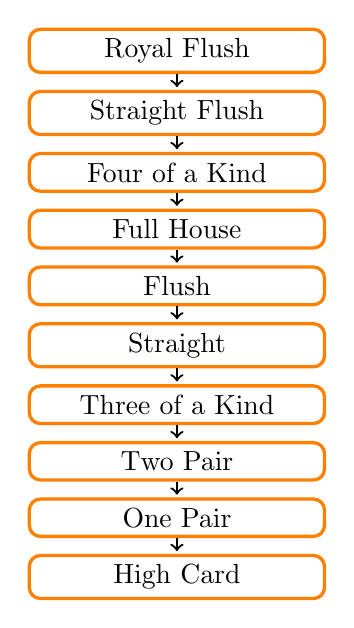
\begin{tikzpicture}
  [node distance=.2cm,
  start chain=going below,]
     \node[punktchain, join] (RoyalFlush) {Royal Flush};
     \node[punktchain, join] (StraightFlush){Straight Flush};
     \node[punktchain, join] (FourofaKind){Four of a Kind};
     \node[punktchain, join] (FullHouse){Full House};
     \node[punktchain, join](Flush){Flush};
     \node[punktchain, join](Straight){Straight};
     \node[punktchain, join](ThreeofaKind){Three of a Kind};
     \node[punktchain, join](TwoPair){Two Pair};
     \node[punktchain, join](OnePair){One Pair};
     \node[punktchain, join](HighCard){High Card};

   \end{tikzpicture}
   }
   \caption{(a) shows the wrong representation and (b) shows the correct representation to follow when playing a game of poker}
   \label{fig:pr}
   \end{figure}
\end{document}